\chapter{Umsetzung}
\label{umsetzung}

Die Umsetzung der vorliegenden Problemstellung wird mit Hilfe des in \vref{kdd} vorgestellten KDD-Prozesses durchgeführt. Anhand der erlernten Grundlagen und Methoden der einzelnen Prozessschritte, werden diese sukzessive durchlaufen, um eine möglichst exakte Modellierung der Funktion zu realisieren. Zunächst werden die relevanten Daten in \vref{ds} selektiert, anschließend aufbereitet (vgl. \vref{dv}) und in das für die Regressionsanalyse passende Format transformiert (vgl. \vref{dt}). Im darauf folgenden Schritt des Data Minings wird die Funktion unter der Betrachtung des Winkels und der Distanz, als auch in Bezug auf die Koordinaten des Schusses anhand der Regression (vgl. \vref{fm}) modelliert. Abschließend werden die aus \gls{matlab} gewonnenen Ergebnisse interpretiert und evaluiert, um eine fundierte Entscheidung über die Auswahl eines Modells treffen zu können.

\section{Datenselektion}
\subsection{Datenvorverarbeitung}
\label{aufbereitung}
\glqq Da die Zieldaten aus den Datenquellen lediglich extrahiert werden, ist im Rahmen der Datenvorverarbeitung die Qualität des Zieldatenbestandes zu untersuchen und – sofern nötig – dieser durch den Einsatz geeigneter Verfahren zu verbessern.\grqq\seFootcite{}{S. 9}{Cleve.2014}

Diese essentielle Phase verfolgt das Ziel, die unstrukturierten und zunächst nutzlos scheinenden, selektierten Rohdaten, in qualitativ hochwertigere Daten umzuwandeln, um diese der passenden \gls{dm}-Methode in einem geeigneten Format bereitstellen zu können. Die Struktur und das Format müssen perfekt auf die vorliegende Aufgabe passen, ansonsten führt die geringe Qualität der Daten zu schlechten bzw. falschen Resultaten, bis hin zu Laufzeitfehlern.\seFootcite{Vgl.}{S. 10-11}{Garcia.2015} Es gilt auch hier das Prinzip: GIGO – garbage in, garbage out.\seFootcite{Vgl.}{S. 197}{Cleve.2014} Die oftmals schlechte Qualität der (Roh-)Daten ist durch \textit{fehlende, ungenaue, inkonsistente bzw. widersprüchliche} Daten zu begründen.\seFootcite{Vgl.}{S. 84}{Han.2012}\seFootcite{Vgl.}{S. 196}{Cleve.2014} Im Folgenden werden dazu einige Ursachen beispielhaft aufgeführt.

Ungenaue bzw. falsche Daten können schon bei der Erhebung entstehen, wenn ein falsches Datenerhebungsinstrument ausgewählt wird. Bei Stichproben sollte die Gesamtmenge so präzise wie möglich widergespiegelt werden, um die Datenakkuratesse nicht zu gefährden.\seFootcite{Vgl.}{S. 25}{Fahrmeir.2007} Weiterhin können technische und menschliche Fehler zu ungenauen Daten führen, indem Personen beispielsweise ihre persönlichen Informationen bei einer Befragung absichtlich verschleiern (z.B. Standardwert für Geburtsdatum 1. Januar), wobei man diese Problematik auch als \textit{\glqq disguised missing data\grqq}~bezeichnet.\seFootcite{Vgl.}{S. 84}{Han.2012}\seFootcite{Vgl.}{S. 24}{Fahrmeir.2007}\seFootcite{Vgl.}{S. 196}{Cleve.2014} Neben der falschen subjektiven Einschätzung des Menschen bei der Erhebung, können auch von einem technischem Blickwinkel ungenaue Daten ermittelt werden, wie z.B. durch (teils-)defekte Sensoren.\enlargethispage{\baselineskip}  Nicht zuletzt können Daten bei einem Transfer verfälscht werden bzw. sogar verloren gehen.\seFootcite{Vgl.}{S. 84}{Han.2012}

Fehlende Daten lassen sich einerseits durch technische Mängel begründen, andererseits auch durch die Tatsache, dass bestimmte Attribute schlichtweg von Beginn an bei der Erhebung nicht beachtet wurden oder durch bestimmte Restriktionen nicht verfügbar waren.\seFootcite{Vgl.}{S. 84-85}{Han.2012}

Die aufgezeigten Beispiele spiegeln nur einen kleinen Teil möglicher Ursachen wider und sollen die Bedeutsamkeit dieser Phase für den Data-Mining-Prozess aufzeigen. Die Datenvorbereitung stellt dabei einige leistungsstarke Werkzeuge zur Verfügung, um die Datenqualität nachhaltig zu verbessern:\seFootcite{Vgl.}{S. 11 ff}{Garcia.2015}\seFootcite{Vgl.}{S. 196 ff}{Cleve.2014}\seFootcite{Vgl.}{S. 84 ff}{Han.2012}

\begin{itemize}
\item \textbf{Data Cleaning}: In diesem Schritt werden die Daten bereinigt, indem beispielsweise \textit{fehlerhafte} oder \textit{störende} Daten korrigiert werden (siehe \vref{dc}).

\item \textbf{Data Integration}: Diese Phase beschäftigt sich mit der fehlerfreien Zusammenführung von Daten, da diese oftmals aus mehreren unterschiedlichen Quellen stammen (siehe \vref{di}).

\item \textbf{Data Reduction}: Um die Algorithmen der Data Mining Methoden nutzen zu können, muss die exorbitante Datenmenge reduziert bzw. komprimiert werden, sodass lange Laufzeiten verhindert beziehungsweise reduziert werden können (siehe \vref{dr}).
\end{itemize}

Auf die in \vref{werkzeuge} vereinfacht dargestellten Werkzeuge und ihre Konzepte, wird in den folgenden Unterkapiteln näher eingegangen.

\begin{figure}[H]
\centering
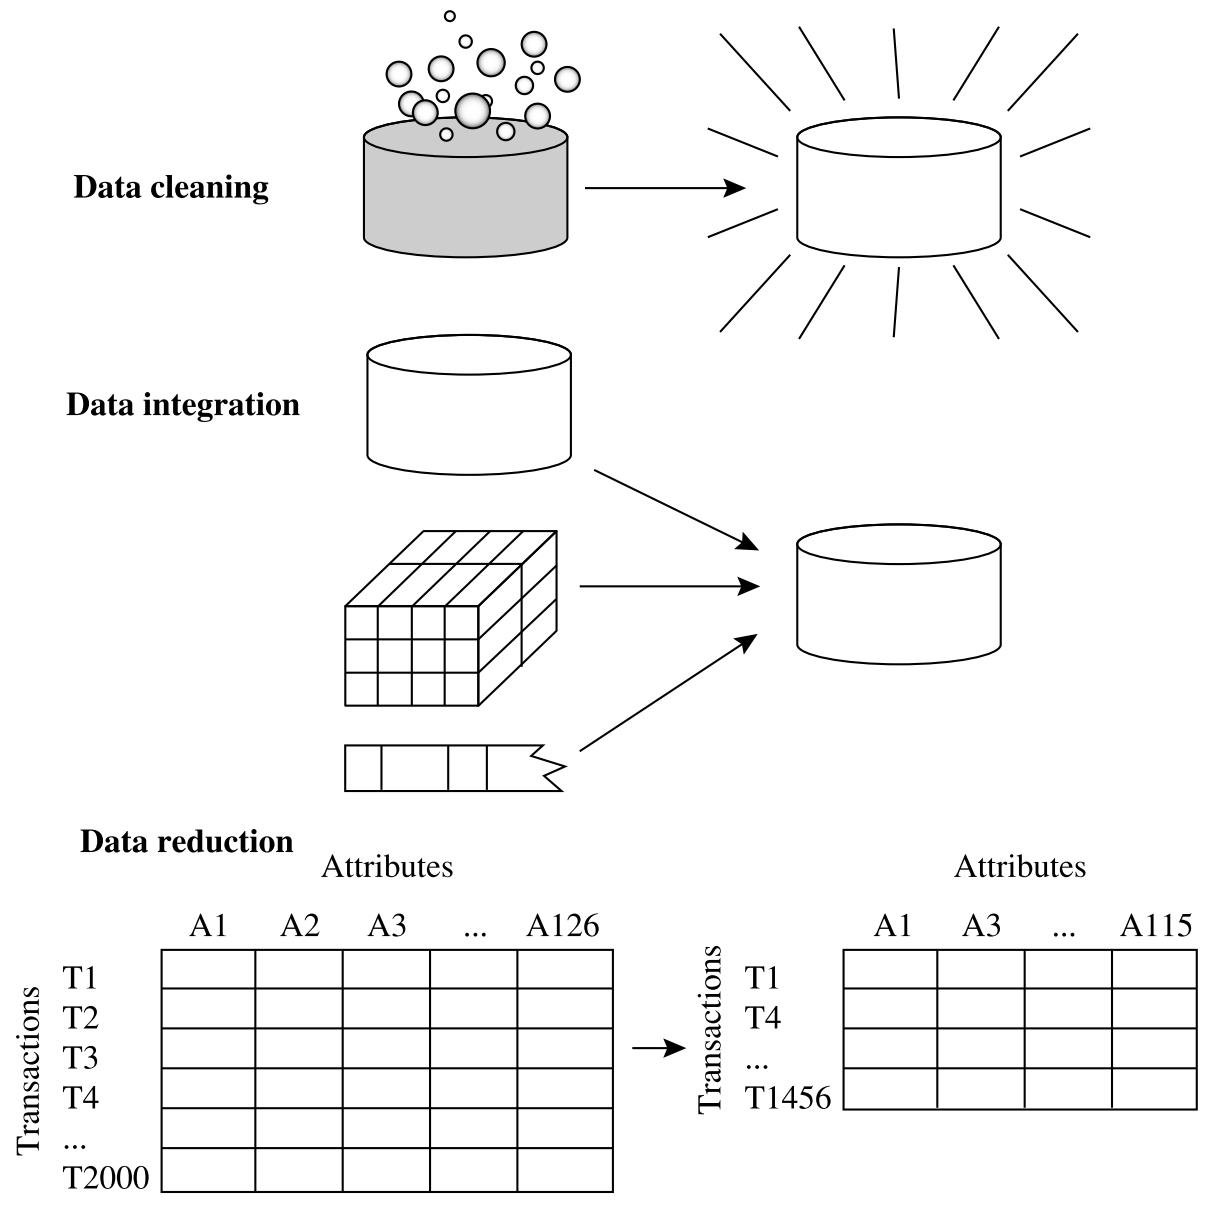
\includegraphics[scale=1.2]{se-wa-jpg/preprocessing}
\caption[Werkzeuge der Datenvorverarbeitung]{Werkzeuge der Datenvorverarbeitung\protect\footnotemark}
\label{werkzeuge}
\end{figure}
\footnotetext{Vgl. Abbildung \textit{Han}, Data Mining: Concepts and techniques, 2012, S. 87}


\subsubsection{Data Cleaning}
\label{dc}
In der realen Welt sind Daten häufig \glqq unvollständig, mit Fehlern oder Ausreißern behaftet oder sogar inkonsistent.\grqq\seFootcite{}{S. 199}{Cleve.2014} Um Fehler oder gar falsche Resultate im Data-Mining-Prozess frühzeitig zu vermeiden, ist es von großer Bedeutung, die Datenmengen zu bereinigen. Der Fokus sollte hierbei auf der Informationsneutralität liegen. Das bedeutet, es sollen möglichst keine neuen Informationen hinzugefügt werden, die das reale Abbild verzerren oder verfälschen können.\seFootcite{Vgl.}{S. 199-200}{Cleve.2014} Folgende Problemarten gilt es zu behandeln:

\paragraph{Fehlende Daten} 
Dem Datenanalyst stehen einige Möglichkeiten zur Verfügung, um auf fehlende Daten zu reagieren:\seFootcite{Vgl.}{S. 88-90}{Han.2012}\seFootcite{Vgl.}{S. 200-201}{Cleve.2014}

\begin{itemize}
\item \textit{Attribut ignorieren}
\\ Der Datensatz mit dem fehlenden Attribut wird gänzlich ignoriert oder gelöscht. Jedoch können dadurch wichtige Informationen für die Datenanalyse verloren gehen, wodurch dieses Verfahren nur bei Datensätzen mit mehreren Lücken angewandt werden sollte.

\item \textit{Manuelles Einfügen}
\\ Besitzt der Datenanalyst das nötige Wissen, kann dieser einzelne Datensätze nachträglich manuell einfügen. Dieser Vorgang entwickelt sich schnell zu einem sehr zeitaufwändigen und schwer zu realisierenden Vorgang, der aufgrund des Mangels an Ressourcen (personeller wie auch zeitlicher) nicht zu realisieren ist, sobald die Datenmenge wächst (z.B. Nachtrag von 500 Kundendaten per Hand).

\item \textit{Globale Konstante}
\\ Den fehlenden Wert durch eine globale Konstante (auch als Standardwert bezeichnet) zu ersetzen, ist sinnvoll, wenn auch ein leeres Feld als Information angesehen wird. Beispiele für Konstanten wären \textit{unbekannt} oder \textit{minus unendlich}.

\item \textit{Durchschnittswert}
\\ Handelt es sich bei dem fehlenden Attribut um einen metrischen Wert, so kann der Durchschnittswert aller Einträge als Ersatz verwendet werden. Der Durchschnittswert bietet sich als äußerst einfache Möglichkeit, wenn die Daten klassifiziert werden können und die Berechnung nur auf Datensätzen der selben Klasse angewandt wird. Die Methode der \gls{knn}\seFootcite{Vgl.}{S. 76}{Garcia.2015} steht zur Verfügung, wenn keine Klassen vorhanden sind. Hierbei wird der Durchschnitt, der dem aktuellen Datensatz ähnlichsten Werte benutzt.

\item \textit{Wahrscheinlichster oder häufigster Wert}
\\ Durch statistische Methoden kann der wahrscheinlichste Wert für das fehlende Attribut ermittelt werden, jedoch sollte diese Angleichung begründet sein. Bei nicht numerischen Werten kann als weitere Möglichkeit auch der häufigste Wert als Ersatz für das fehlende Attribut verwendet werden.
\end{itemize}

\paragraph{Verrauschte Daten und Ausreißer}
\label{outlierchapter}
Durch ungenaue Messwerte oder falsche Schätzungen entstehen die sogenannten \textit{verrauschten Daten}.\footnote{Im englischen Sprachgebrauch als \textit{noisy data} bekannt.} Um diese bereinigen zu können, stehen dem Datenanalyst einige Verfahren zur Verfügung, durch welche diese fehlerbehafteten Daten angeglichen werden können.\footnote{Auch als \textit{smoothing} bekannt.} Als \textit{Ausreißer} bezeichnet man dabei Daten, die erheblich von den anderen Daten abweichen oder außerhalb eines Wertebereiches (z.B. $0<x<100$) liegen.\seFootcite{Vgl.}{S. 89-90}{Han.2012} Beispielsweise liegen bei einer Befragung Daten von 30- bis 50-Jährigen vor, darunter auch einer von einem 90-Jährigen, könnte es sich hierbei um einen Ausreißer handeln, aber auch um einen fehlerhaften Datensatz.\seFootcite{Vgl.}{S. 196}{Cleve.2014} \glqq Ob solche Ausreißer für das Data Mining ausgeblendet oder adaptiert werden sollten oder besser doch im Originalzustand zu verwenden sind, hängt vom konkreten Kontext ab.\grqq\seFootcite{}{S. 196}{Cleve.2014}


\begin{itemize}

\item \textit{Klasseneinteilung (bining)}
\\ Durch die Gruppierung verrauschter Daten in Klassen, können diese beispielsweise durch den Mittelwert oder die naheliegenden Grenzwerte ersetzt werden. 

\item \gls{regression}
\\ Die Darstellung der Daten in Form einer mathematischen Funktion, bietet die Möglichkeit, fehlerbehaftete Daten  durch die berechneten Funktionswerte zu ersetzen. Für zwei Abhängigkeiten zwischen zwei Attributen steht hierbei neben der \textit{linearen Regression}, auch die \textit{multiple lineare Regression} für mehrere Attribute als Werkzeuge zur Verfügung (weiterführende Ausarbeitung zur Regressionsanalyse siehe \vref{ra}). 

\item \textit{Verbundbildung (clustering)}
\\ Eine der einfachsten Möglichkeiten um Ausreißer zu erkennen, bietet die Verbundbildung, auch \gls{clustering} genannt. Hierbei werden ähnliche Daten, wie in \vref{outlier} dargestellt, zu \textit{Clustern} zusammengeführt, wodurch sich die Ausreißer direkt identifizieren lassen.

\begin{figure}[H]
\centering
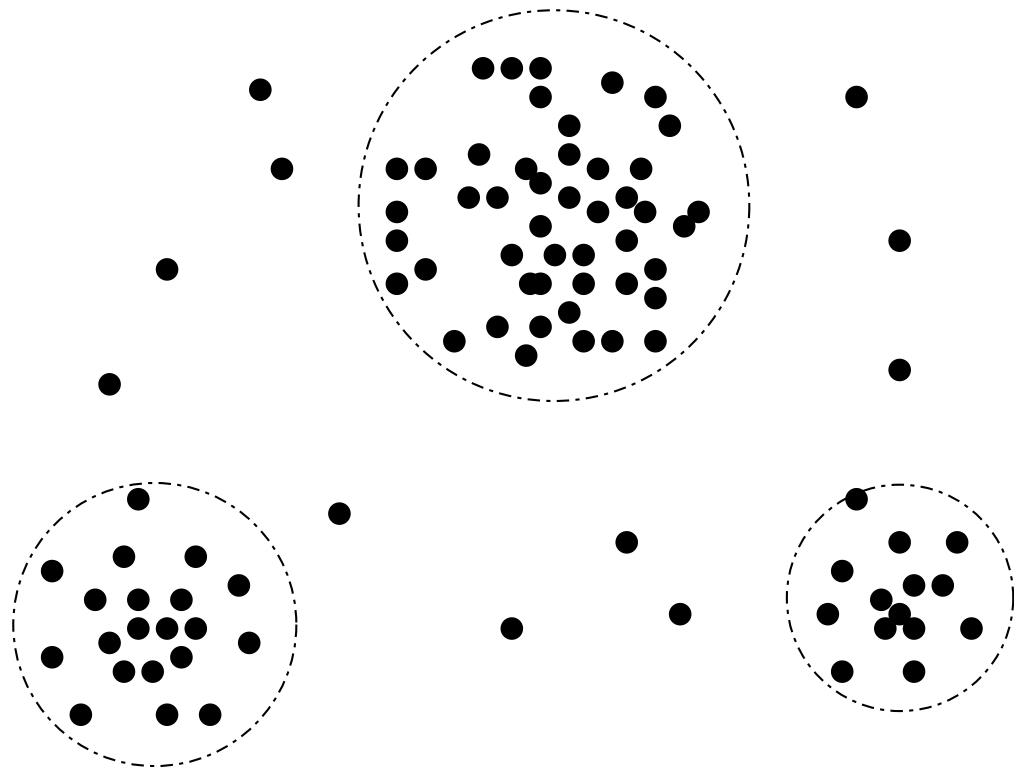
\includegraphics[scale=1.2]{se-wa-jpg/outlier}
\caption[Outlierdetection mittels Clustering]{Outlierdetection mittels Clustering\protect\footnotemark}
\label{outlier}
\end{figure}
\footnotetext{Vgl. Abbildung \textit{Han}, Data Mining: Concepts and techniques, 2012, S. 91}
\end{itemize}

\paragraph{Falsche und inkonsistente Daten}
Bei falschen bzw. inkonsistenten Daten ergeben sich prinzipiell zwei Möglichkeiten zur Korrekturbehandlung. Einerseits können der Datensatz oder bestimmte Attribute durch \textit{Löschen} entfernt werden, wobei jedoch die Gefahr einer zu großen Reduktion des Datenbestandes entsteht und relevante Informationen für das Data Mining verloren gehen könnten. Die zweite Korrekturvariante versucht den inkonsistenten Datensatz, durch die \textit{Zuhilfenahme anderer Datensätze}, sinnvoll zu ersetzen. Sollte eine Unterscheidung zwischen \textit{falsch} und \textit{richtig} nicht möglich sein, wären beim Löschen immer mindestens zwei Datensätze betroffen.\seFootcite{Vgl.}{S. 203-204}{Cleve.2014}

\subsubsection{Data Integration}
\label{di}
Bei Data-Mining-Projekten ist oftmals die Integration mehrerer Datenbestände aus unterschiedlichen Quellen erforderlich. Diese Phase sollte mit äußerster Sorgfalt durchgeführt werden, um frühzeitig redundante und inkonsistente Datensätze zu vermeiden, wodurch die Genauigkeit und Geschwindigkeit der nachfolgenden Data Mining Algorithmen nicht gefährdet wird.\seFootcite{Vgl.}{S. 93-94}{Han.2012} Folgende Punkte gilt es bei der Datenintegration zu beachten:

\begin{itemize}
\item \textbf{Identifikationsproblem von Entitäten}:
\\ Bei der Datenintegration aus multiplen Datenquellen, wie beispielsweise Datenbanken oder Dokumenten, stellt die Schema-Integration wie auch die Objektanpassungen eine schwierige Herausforderung dar. Der Datenanalyst muss sicherstellen, dass zum Beispiel das Attribut \textit{kunden\_nummer} aus der einen Datenquelle, die selbe Referenz besitzt, wie das Attribut \textit{kunden\_id} aus einer anderen und es sich folglich um das selbe Attribut handelt. Dies wird allgemein als \textit{Problem Identification Problem} bezeichnet.\seFootcite{Vgl.}{S. 199}{Cleve.2014}\seFootcite{Vgl.}{S. 94}{Han.2012} Die Metadaten der Attribute beinhalten Informationen, wie \textit{Name, Bedeutung, Datentyp, Wertebereich, uvm.} und können durch Abgleich derer zu einer Vermeidung von Fehlern bei der Integration beitragen. Weiterhin muss gesondert auf die \textit{Datenstruktur} geachtet werden, um keine referentiellen Abhängigkeiten bzw. Beziehungen zwischen den Daten zu zerstören.\seFootcite{Vgl.}{S. 94}{Han.2012} 

\item \textbf{Redundanzen bei Attributen}:
\\ Ein Attribut, welches durch ein anderes Attribut ableitbar ist -- wie zum Beispiel das Alter vom Geburtsjahr berechnet werden kann -- wird als redundant bezeichnet. Die Vielzahl von Redundanzen führt zu unnötig großen Datenmengen, die wiederum die Performanz sowie die Resultate eines Data Mining Algorithmus negativ beeinträchtigen können.\seFootcite{Vgl.}{S.41}{Garcia.2015} Folglich sollte diese Problematik durch die Anwendung von statistischen Verfahren, in Form der Korrelationsanalyse, dezidiert behandelt werden. Für numerische Werte ist dabei der Einsatz von Korrelationskoeffizienten und Kovarianzen hilfreich. Um die Implikation zweier Attribute einer nominalen Datenmenge\footnote{Rein qualitative Merkmalsausprägungen ohne natürliche Rangordnung (wie z.B. das Geschlecht).} bestimmen zu können, verwendet man in der Regel den $\chi^2$(\textit{Chi-Quadrate})-Test.\seFootcite{Vgl.}{S. 95.}{Han.2012}\seFootcite{Vgl.}{S. 41}{Garcia.2015}\seFootcite{Vgl.}{S. 64}{Cleve.2014} 

\item \textbf{Duplikatserkennung}:
\\ Duplikate verkörpern Redundanzen auf Datensatzebene und führen einerseits zu unnötig großen Datenmengen, die sich wiederum auf die Performanz der Algorithmen auswirken. Andererseits führt jedoch auch die verfälschte Gewichtung der mehrfach vorkommenden Datensätze, zu falschen Analyseergebnissen. Ein häufiger Grund stellt dabei die Verwendung von denormalisierten Datenbanktabellen dar.\seFootcite{Vgl.}{S. 98}{Han.2012}\seFootcite{Vgl.}{S. 43}{Garcia.2015}

\item \textbf{Konflikte bei Attributswerten}:
\\ Hierbei handelt es sich um die unterschiedliche Darstellung, Skalierung und Kodierung von Attributswerten. Beispielsweise kann das Attribut \textit{Gewicht} durch das metrische System oder das britische Maßsystem repräsentiert werden, woraus bei der Zusammenführung von Daten in eine einheitliche Quelle immer wieder Konflikten resultieren.\seFootcite{Vgl.}{S. 99}{Han.2012}\seFootcite{Vgl.}{S. 199}{Cleve.2014} 
\end{itemize}

\subsubsection{Data Reduction}
\label{dr}
Die bereits mehrfach angesprochene Problematik der riesigen Datenmengen bei Data-Mining-Projekten, steigert die Komplexität und vermindert die Effizienz der Algorithmen. Daher strebt die Datenreduktion -- wie die Bezeichnung erkennen lässt -- nach einer reduzierten repräsentativen Teilmenge, welche die Integrität des Originals nicht verliert. Dazu können folgende drei Techniken angewandt werden:\seFootcite{Vgl.}{S. 147 ff}{Garcia.2015}\seFootcite{Vgl.}{S. 99-100}{Han.2012}\seFootcite{Vgl.}{S. 206-208}{Cleve.2014} 

\begin{enumerate}

\item Dimensionsreduktion 

\item Datenkompression

\item Numerische Datenreduktion

\end{enumerate}

\paragraph{Dimensionsreduktion}
Hierbei bleiben irrelevante Attribute des Datensatzes unberücksichtigt und nur für die Analyse relevante Daten werden miteinbezogen. Allgemein empfehlen sich dafür zwei Verfahren: Bei der schrittweisen \textit{Vorwärtsauswahl} werden wesentliche Attribute einer sukzessiv wachsenden Zielmenge zugeordnet. Im Gegensatz dazu werden bei der \textit{Rückwärtseliminierung} die uninteressanten Daten schrittweise aus der Zielmenge eliminiert.\seFootcite{Vgl.}{S. 206}{Cleve.2014} 

\paragraph{Datenkompression}
\label{datenkompression}
Bei dieser Technik wird durch Transformation oder Codierung versucht, eine Reduktion der Datenmenge zu erreichen. Fasst man beispielsweise die einzelnen Attribute \textit{Tag, Monat und Jahr} zu einem neuen Attribut \textit{Datum} zusammen, können Datensätze komprimiert werden.\seFootcite{Vgl.}{S. 207}{Cleve.2014}
 
\paragraph{Numerische Datenreduktion}
Statt die gesamte Datenmenge für die Analyse heranzuziehen, wird innerhalb der numerischen Datenreduktion eine repräsentative Teilmenge -- in Form einer Stichprobe -- für das \gls{dm} genutzt. Im Vordergrund steht hierbei die passende Auswahl unterschiedlicher Stichprobeverfahren, wie der \textit{zufälligen Stichprobe} oder der \textit{repräsentativen Stichprobe}, woraus jedoch kein verzerrtes Abbild der Daten resultieren darf.\seFootcite{Vgl.}{S. 25-27}{Fahrmeir.2007}\seFootcite{Vgl.}{S. 207}{Cleve.2014}
\subsection{Datentransformation}
\label{dt}
Nachdem die (Roh-)Daten selektiert, bereinigt und auf eine relevante Zielmenge reduziert wurden, müssen diese noch in eine adaptierte Form für die Algorithmen des Data Minings transformiert werden.\seFootcite{Vgl.}{S. 112}{Han.2012} Oftmals müssen sogar neue Attribute aus einem Datensatz kreiert werden, da dieser nicht in geeigneter Struktur für das Data-Mining-Verfahren vorliegt.\seFootcite{Vgl.}{S. 48}{Garcia.2015} Dazu gibt es eine Reihe an unterschiedlichen Transformationsmöglichkeiten, wobei in dieser Arbeit ein Auszug der relevanten Methoden vorgestellt werden soll:

\paragraph{Codierung}
Liegen beispielsweise Attribute mit einer ordinalen Ausprägung vor (wie \textit{sehr groß, groß, mittel und klein}), müssen diese bei einer Verwendung des \gls{knn}-Algorithmus in numerische Werte transformiert werden (Werte zwischen 0 und 1). Hierbei würde sich folgende Codierung für das Attribut \textit{Körpergröße} anbieten:\seFootcite{Vgl.}{S. 210}{Cleve.2014}

\begin{itemize}
\item \textit{sehr groß} $\rightarrow$ 1
\item \textit{groß} $\rightarrow$ 0,66
\item \textit{mittel} $\rightarrow$ 0,33
\item \textit{klein} $\rightarrow$ 0
\end{itemize}

Die Ordnungsrelation, hier \textit{sehr groß > groß > ...}, darf dabei jedoch nicht verloren gehen. In Abhängigkeit zu dem jeweiligen Verfahren, müssen Daten, so wie dies bei Maßeinheiten immer wieder der Fall ist, oftmals kodiert werden.\seFootcite{Vgl.}{S. 211}{Cleve.2014}

\paragraph{Normalisierung und Skalierung}
Unterschiedliche Maßeinheiten -- wie \textit{Körpergröße} und \textit{Körpergewicht} -- können die Datenanalyse negativ beeinflussen und müssen daher in eine einheitliche Skalierung transformiert werden, um eine gleiche Gewichtung aller Attribute zu erreichen. Man bedient sich hierbei in der Regel an der \textit{Min-Max-Normalisierung} (siehe \vref{minmax}) oder der \textit{Z-Transformation}, um numerische Werte auf ein [0,1] Intervall zu normieren.\seFootcite{Vgl.}{S. 114}{Han.2012}\seFootcite{Vgl.}{S. 212}{Cleve.2014}

\begin{figure}[H]
\begin{equation}
x_{neu} = \frac{x - min(x_i)}{max(x_i) - min(x_i)}
\end{equation}
\caption{Min-Max-Normalisierung}
\label{minmax}
\end{figure}

\paragraph{Datenaggregation}
Nicht nur aus Sicht der Datenkompression (vgl. \vref{datenkompression}) ist die Datenaggregation erforderlich. Vielmehr \glqq kann die Aggregation aus inhaltlichen Gründen sinnvoll sein.\grqq\seFootcite{}{S. 214}{Cleve.2014} Wenn Daten auf einer zu detaillierten Ebene vorliegen -- wie beispielsweise Einwohnerzahlen von Stadtteilen -- müssen diese für einen Städtevergleich erst summiert werden, um bundesweite Aussagen treffen zu können. Je nach Kontext können verschiedene Aggregationsmethoden (wie z.B. Summenbildung, Durchschnitt, usw.) für die Transformation zu einem einzigen Wert angewendet werden.\seFootcite{Vgl.}{S. 112}{Han.2012}

\paragraph{Datenglättung}
Die bereits in \vref{outlierchapter} vorgestellten Techniken zur Bereinigung von verrauschten Daten und Ausreißern, finden auch bei der Transformation ihre Verwendung. Die Datenglättung strebt nach einer reduzierten Datenmenge, in welcher jeder numerische Wert durch einen idealisierten Wert, wie beispielsweise der \textit{\gls{regression}}, ersetzt wird.\seFootcite{Vgl.}{S. 214-215}{Cleve.2014}
\subsection{Data-Mining-Methoden}
\label{dmmethoden}

Nachdem die Daten in geeigneter Form vorliegen, kommt das eigentliche Herzstück des \gls{kdd}-Prozesses -- das \textit{Data Mining} -- zum Tragen. In diesem Schritt wird zu nächst überprüft, welche grundlegende Data-Mining-Aufgabe es zu lösen gilt, um anschließend ein passendes Analyseverfahren zur Identifizierung von Mustern und Zusammenhängen auswählen zu können.\seFootcite{Vgl.}{S. 10}{Cleve.2014} Die interdisziplinäre Wissenschaft des Data Minings umfasst bewährte Techniken aus mehreren Forschungsgebieten, welche auf verschiedenste Problemfälle der Realität, wie Zeitreihenanalysen, Funktionsmodellierungen, Klassifikation uvm., angewendet werden können. Grundsätzlich basieren fast alle Analyseverfahren auf der Mathematik, insbesondere der Statistik.\seFootcite{Vgl.}{S. 12}{Cleve.2014} Im Allgemeinen unterteilt man die Data-Mining-Methoden in zwei Kategorien: \textit{Prognose} und \textit{Beschreibung}. Hierzu gibt \vref{dmmethods} einen Überblick über die Einteilung der etablierten Methoden, welche im Folgenden kurz aufgeführt werden.

\paragraph{Prognose:} In dem Bereich der Prognose unterscheidet man zwischen zwei Gruppen: \textit{statistische Methoden} und \textit{symbolische Methoden}. Letztere versuchen das Wissen durch Symbolik und Verknüpfung, auf einer leichter interpretierbaren Ebene für Menschen, zu vermitteln. Im Gegensatz dazu, repräsentieren statistische Methoden das Wissen mit Hilfe der Erstellung von mathematischen Modellen.\seFootcite{Vgl.}{S. 3}{Garcia.2015} Die am häufigsten angewendeten statistischen Methoden sind folgende:\seFootcite{Vgl.}{S. 3-5}{Garcia.2015}\seFootcite{Vgl.}{S. 23-24}{Han.2012}

\begin{itemize}
\item \textit{Regressionsanalyse}
\\ Die älteste \gls{dm}-Methode dient zur Funktionsmodellierung von einer abhängigen oder mehreren unabhängigen Variablen. Die Form der Funktion wird dabei durch das ausgewählte Verfahren, beispielsweise \textit{lineare oder quadratische Regression}, bestimmt und kann anhand bestimmter Parameter validiert werden, wie \glqq gut\grqq~diese zu den eingebrachten Daten passt.\seFootcite{Vgl.}{S. 3}{Garcia.2015}

\item \textit{(Künstliche)} \gls{nn}
\\ In diesem Teilbereich der künstlichen Intelligenz wird versucht, einen Wissensspeicher zu kreieren, der ähnlich unserem leistungsfähigen Gehirn funktioniert. Hierbei werden die biologischen Elemente und Vorgehensweise des Gehirns, in Form von \textit{Neuronen}, in die Welt des Computers übertragen. Durch gerichtete und gewichtete Verbindungen sind diese Neuronen untereinander verknüpft und bilden so ein gemeinsames Netz für die Informationsverarbeitung.\seFootcite{Vgl.}{S. 47}{Cleve.2014}

\item \gls{svm}
\\ Die auf \gls{ml} basierende Methode versucht Objekte zu klassifizieren. Dabei werden alle Objekte als Vektoren in einem Raum dargestellt und durch sogenannte \textit{Hyperebenen} (fungieren als Trennflächen) geteilt, um eine möglichst zuverlässige Zuordnung der Daten in vordefinierte Klassen zu erreichen.\seFootcite{Vgl.}{S. 313}{Aggarwal.2015}
\end{itemize}

Im Bereich der symbolischen Methoden hat sich die Technik des \textit{Entscheidungsbaumes} etabliert. Sie dient ebenfalls der Klassifizierung von Objekten, indem innerhalb jedes Iterationsschrittes das am \textit{besten} zu klassifizierende Attribut gefunden wird, um die Daten daran aufzusplitten. Durch dieses Verfahren entsteht ein Entscheidungsbaum, von dem Regeln, wie \textit{If-Else-Zweige}, abgeleitet werden können.\seFootcite{Vgl.}{S. 5}{Garcia.2015}

\paragraph{Beschreibung:}

\begin{itemize}
\item \textit{Clustering}
\\ Im Gegensatz zur Klassifizierung sind bei der Methode des Clustering zuvor keine Klassen bzw. Gruppen definiert. Dieses weitverbreitete Werkzeug im Bereich des Data Minings versucht Daten in sogenannte \textit{Cluster} zu unterteilen, wobei die Elemente dieser Gruppen sich möglichst ähnlich (\textit{homogen}), jedoch auch gleichzeitig von den anderen Clustern deutlich zu unterscheiden sein sollten (\textit{heterogen}).\seFootcite{Vgl.}{S. 3}{Anderberg.2014}
\enlargethispage{\baselineskip} 
\item \textit{Assoziationsanalyse}
\\ Diese Methode versucht Wissen durch assoziative Beziehungen zwischen den Daten herzuleiten. Das einfachste Beispiel hierfür wäre im Einzelhandelsbereich: \glqq Wenn ein Kunde Produkt A kauft, würde dieser auch Produkt B kaufen.\grqq~Durch diese extrahierten Muster, können wiederum Regeln abgeleitet werden.
\end{itemize}


\paragraph{Visualisierung als Werkzeug:}
Nicht zuletzt ist die Visualisierung unerlässlich für den Erfolg eines Data-Mining-Projektes. Die Resultate werden oftmals zur Entscheidungsfindung herangezogen, wobei die Entscheidungsträger nicht immer direkt am Prozess beteiligt sind. Die Ergebnisse müssen folglich in einer anschaulichen und nachvollziehbaren Form dargestellt werden, um Vertrauen und Akzeptanz in die Resultate zugewinnen.\seFootcite{Vgl.}{S. 14}{Cleve.2014} Weiterhin kann die Visualisierung auch schon in der Datenvorverarbeitung genutzt werden oder als eigenständige Methode innerhalb des Data Minings, da sich häufig erst Zusammenhänge zwischen den Attributen durch die Darstellung der Daten erkennen lassen.\seFootcite{Vgl.}{S. 14}{Cleve.2014}

\paragraph{Auswahl der Methode:}
Für die Modellierung einer Funktion zur Berechnung der Wahrscheinlichkeit eines Torerfolges im Fußball (auch bekannt unter dem Begriff \textit{Expected Goals}), kann die passende Data-Mining-Methode aus der \vref{dmmethods} ausgewählt werden. Der zu erwartende Torerfolg soll folglich prognostiziert und durch ein mathematisches Modell repräsentiert werden. Unter den statistischen Methoden eignet sich für die Modellierung einer Funktion am besten die Regressionsanalyse, da ein Torerfolg von mehreren Faktoren abhängig ist. Dementsprechend wird dieses Verfahren als Data-Mining-Methode für die Beantwortung der vorliegenden Problemstellung ausgewählt und dessen Bestandteile zunächst in \vref{fm} betrachtet, um diese Technik in der späteren Umsetzung anwenden zu können.	

\begin{sidewaysfigure}
\centering
\includegraphics[scale=0.34]{se-wa-jpg/dmmethods}
\caption[Übersicht: Data-Mining-Methoden]{Übersicht: Data-Mining-Methoden\protect\footnotemark}
\label{dmmethods}	
\footnotetext{Abbildung in Anlehnung an \textit{García} et al., Data preprocessing in data mining, 2015, S. 4.}
\end{sidewaysfigure}
\subsection{Interpretation}
Am Ende des \gls{kdd}-Prozesses steht die Interpretation sowie die Evolution der entdeckten Muster und Beziehungen aus dem Data Mining. Oftmals können Unternehmen keinen Nutzen aus den Analyseverfahren erzielen, da diese häufig irrelevante, triviale, bedeutungslose oder sogar bereits bekannte Daten generieren. Die gewonnenen Muster sollten den folgenden vier Kriterien genügen, um neues Wissen zu repräsentieren:\seFootcite{Vgl.}{S. 11-12}{Cleve.2014}

\begin{enumerate}
\item \textbf{Validität:} Hierbei wird die Gültigkeit des Muster für das gefundene Modell, als auch in Bezug auf neue Daten, in einem objektives Maßstab beschrieben.
\item \textbf{Neuartigkeit:} Das Kriterium beantwortet die Frage, inwiefern das neu erworbene Wissen zu den bisherigen Forschungen steht. Einerseits es kann den Wissensstand ergänzen oder im Widerspruch dazu stehen.
\item \textbf{Nützlichkeit:} Beschreibt das Nutzen, welches für den Anwender durch die Resultate erzielt wurde.
\item \textbf{Verständlichkeit:} Die Ergebnisse des Modells sollten von einem anderen Anwender verstanden werden.
\end{enumerate}

Anhand dieser Anforderungen sollen die späteren Ergebnisse der modellierten Funktionen gemessen werden. Um dabei eine aussagekräftige Interpretation der Ergebnisse treffen zu können, erfordert es ein hohes Maß an Verständnis der vorliegenden Problemstellung. Zu bietet sich ein Team von Experten an, welche die Resultate validieren, sodass eine korrekte Bewertung erzielt wird. Für die Interpretationsphase eignet sich die Verwendung von Werkzeugen, wie der Visualisierung, um schnellen Aufschluss über die gewonnenen Muster und Zusammenhänge zu erlangen. Innerhalb des iterativen \gls{kdd}-Prozesses (siehe \vref{kddpic}) ist ein Rücksprung die vorherigen Phasen typisch.\seFootcite{Vgl.}{S. 11}{Cleve.2014} Meist müssen Daten nochmal nachbereitet, eine andere Data-Mining-Methode ausgewählt oder sogar Daten neu selektiert werden, wenn das gewünschte Ergebnis sich mit der verwendeten Datenbasis nicht erreichen lässt.\seFootcite{Vgl.}{S. 11}{Cleve.2014}